\documentclass{standalone}
\usepackage{tikz}
\usetikzlibrary{patterns, positioning}


\begin{document}
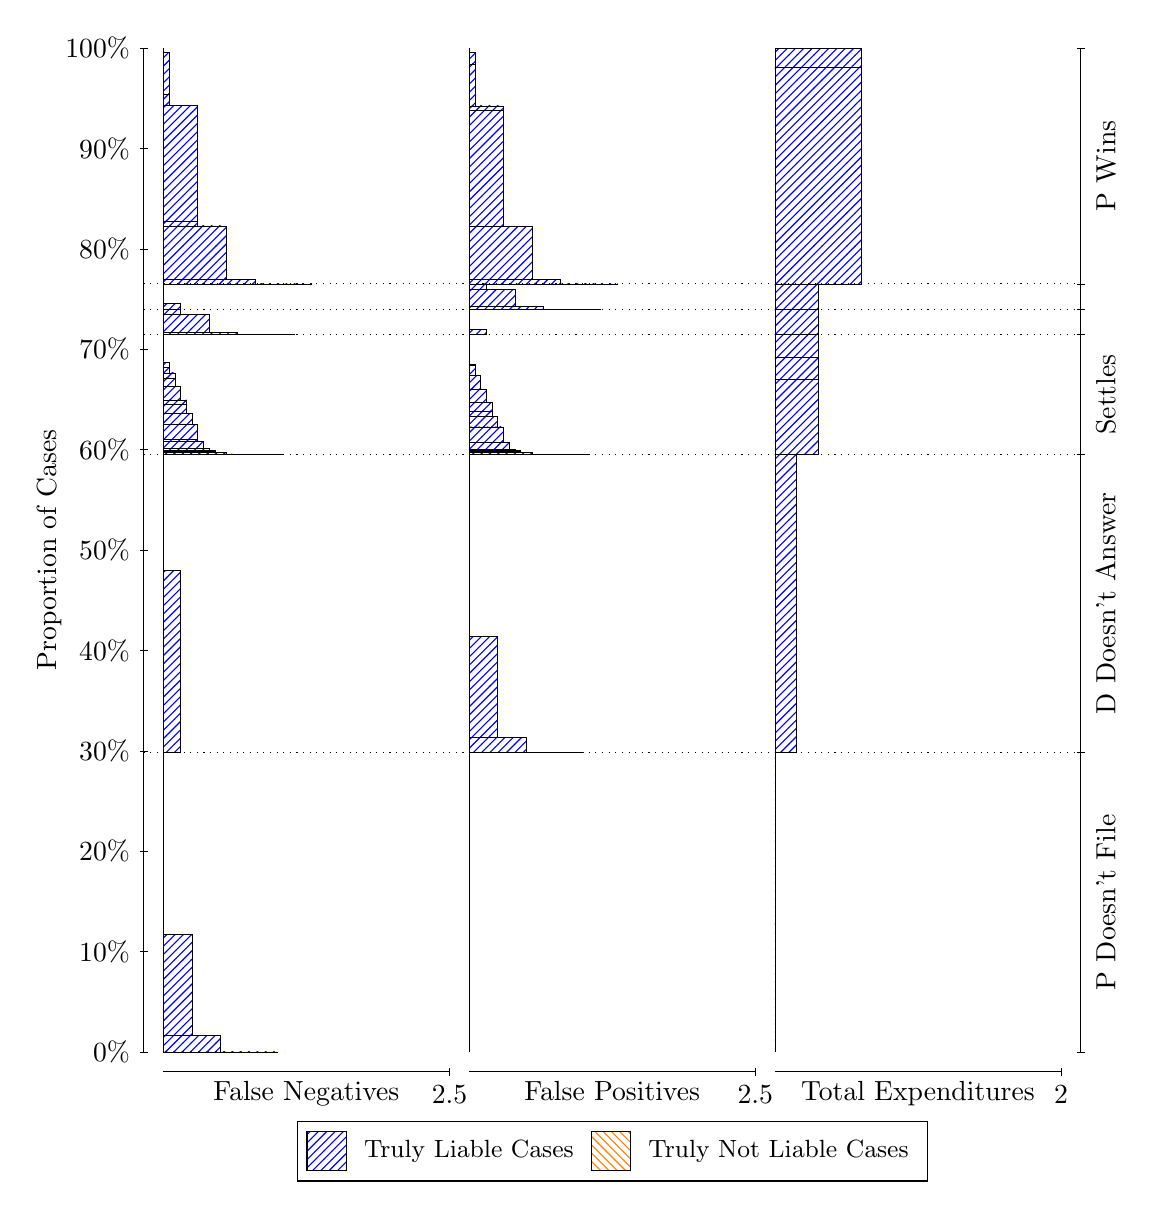
\begin{tikzpicture}
\draw[black, very thin] (1.5,1.75) -- (1.5,14.5);
\node[rotate=90, text=black, anchor=center] at (0.3, 8.125) {Proportion of Cases};
\draw[black, very thin] (1.45,1.75) -- (1.55,1.75);
\node[text=black, anchor=east] at (1.45, 1.75) {0\%};
\draw[black, very thin] (1.45,3.025) -- (1.55,3.025);
\node[text=black, anchor=east] at (1.45, 3.025) {10\%};
\draw[black, very thin] (1.45,4.3) -- (1.55,4.3);
\node[text=black, anchor=east] at (1.45, 4.3) {20\%};
\draw[black, very thin] (1.45,5.575) -- (1.55,5.575);
\node[text=black, anchor=east] at (1.45, 5.575) {30\%};
\draw[black, very thin] (1.45,6.85) -- (1.55,6.85);
\node[text=black, anchor=east] at (1.45, 6.85) {40\%};
\draw[black, very thin] (1.45,8.125) -- (1.55,8.125);
\node[text=black, anchor=east] at (1.45, 8.125) {50\%};
\draw[black, very thin] (1.45,9.4) -- (1.55,9.4);
\node[text=black, anchor=east] at (1.45, 9.4) {60\%};
\draw[black, very thin] (1.45,10.675) -- (1.55,10.675);
\node[text=black, anchor=east] at (1.45, 10.675) {70\%};
\draw[black, very thin] (1.45,11.95) -- (1.55,11.95);
\node[text=black, anchor=east] at (1.45, 11.95) {80\%};
\draw[black, very thin] (1.45,13.225) -- (1.55,13.225);
\node[text=black, anchor=east] at (1.45, 13.225) {90\%};
\draw[black, very thin] (1.45,14.5) -- (1.55,14.5);
\node[text=black, anchor=east] at (1.45, 14.5) {100\%};

\draw[black, very thin] (13.4,1.75) -- (13.4,14.5);
\draw[black, very thin] (13.35,1.75) -- (13.45,1.75);
\node[anchor=west] at (13.35, 1.75) {};
\draw[black, very thin] (13.35,5.553) -- (13.45,5.553);
\node[anchor=west] at (13.35, 5.553) {};
\draw[black, very thin] (13.35,9.3424) -- (13.45,9.3424);
\node[anchor=west] at (13.35, 9.3424) {};
\draw[black, very thin] (13.35,10.859) -- (13.45,10.859);
\node[anchor=west] at (13.35, 10.859) {};
\draw[black, very thin] (13.35,11.185) -- (13.45,11.185);
\node[anchor=west] at (13.35, 11.185) {};
\draw[black, very thin] (13.35,11.506) -- (13.45,11.506);
\node[anchor=west] at (13.35, 11.506) {};
\draw[black, very thin] (13.35,14.5) -- (13.45,14.5);
\node[anchor=west] at (13.35, 14.5) {};

\draw[black, very thin, pattern color=blue, pattern=north east lines] (1.75,1.75) rectangle (3.2033,1.75);
\draw[black, very thin, pattern color=blue, pattern=north east lines] (1.75,1.75) rectangle (2.84,1.7517);
\draw[black, very thin, pattern color=blue, pattern=north east lines] (1.75,1.7517) rectangle (2.4767,1.9583);
\draw[black, very thin, pattern color=blue, pattern=north east lines] (1.75,1.9583) rectangle (2.1133,3.2425);
\draw[black, very thin, pattern color=orange, pattern=north west lines] (1.75,3.2425) rectangle (1.75,3.2425);
\draw[black, very thin, pattern color=blue, pattern=north east lines] (1.75,3.2425) rectangle (1.75,5.553);
\draw[black, very thin, pattern color=blue, pattern=north east lines] (1.75,5.553) rectangle (1.968,7.8643);
\draw[black, very thin, pattern color=orange, pattern=north west lines] (1.75,7.8643) rectangle (1.75,7.8643);
\draw[black, very thin, pattern color=blue, pattern=north east lines] (1.75,7.8643) rectangle (1.75,9.3424);
\draw[black, very thin, pattern color=blue, pattern=north east lines] (1.75,9.3424) rectangle (3.276,9.3424);
\draw[black, very thin, pattern color=blue, pattern=north east lines] (1.75,9.3424) rectangle (3.1307,9.3424);
\draw[black, very thin, pattern color=blue, pattern=north east lines] (1.75,9.3424) rectangle (2.9853,9.3424);
\draw[black, very thin, pattern color=blue, pattern=north east lines] (1.75,9.3424) rectangle (2.9127,9.3424);
\draw[black, very thin, pattern color=blue, pattern=north east lines] (1.75,9.3424) rectangle (2.84,9.3424);
\draw[black, very thin, pattern color=blue, pattern=north east lines] (1.75,9.3424) rectangle (2.7673,9.3425);
\draw[black, very thin, pattern color=blue, pattern=north east lines] (1.75,9.3425) rectangle (2.6947,9.3426);
\draw[black, very thin, pattern color=blue, pattern=north east lines] (1.75,9.3426) rectangle (2.622,9.3462);
\draw[black, very thin, pattern color=blue, pattern=north east lines] (1.75,9.3462) rectangle (2.5493,9.3653);
\draw[black, very thin, pattern color=blue, pattern=north east lines] (1.75,9.3653) rectangle (2.4767,9.3689);
\draw[black, very thin, pattern color=blue, pattern=north east lines] (1.75,9.3689) rectangle (2.404,9.3744);
\draw[black, very thin, pattern color=blue, pattern=north east lines] (1.75,9.3744) rectangle (2.404,9.3915);
\draw[black, very thin, pattern color=blue, pattern=north east lines] (1.75,9.3915) rectangle (2.3313,9.4127);
\draw[black, very thin, pattern color=blue, pattern=north east lines] (1.75,9.4127) rectangle (2.2587,9.5023);
\draw[black, very thin, pattern color=blue, pattern=north east lines] (1.75,9.5023) rectangle (2.186,9.5336);
\draw[black, very thin, pattern color=blue, pattern=north east lines] (1.75,9.5336) rectangle (2.186,9.7242);
\draw[black, very thin, pattern color=blue, pattern=north east lines] (1.75,9.7242) rectangle (2.1133,9.858);
\draw[black, very thin, pattern color=blue, pattern=north east lines] (1.75,9.858) rectangle (2.0407,9.9705);
\draw[black, very thin, pattern color=blue, pattern=north east lines] (1.75,9.9705) rectangle (2.0407,10.032);
\draw[black, very thin, pattern color=blue, pattern=north east lines] (1.75,10.032) rectangle (1.968,10.206);
\draw[black, very thin, pattern color=blue, pattern=north east lines] (1.75,10.206) rectangle (1.8953,10.311);
\draw[black, very thin, pattern color=blue, pattern=north east lines] (1.75,10.311) rectangle (1.8953,10.375);
\draw[black, very thin, pattern color=blue, pattern=north east lines] (1.75,10.375) rectangle (1.8227,10.441);
\draw[black, very thin, pattern color=blue, pattern=north east lines] (1.75,10.441) rectangle (1.8227,10.512);
\draw[black, very thin, pattern color=blue, pattern=north east lines] (1.75,10.512) rectangle (1.75,10.516);
\draw[black, very thin, pattern color=orange, pattern=north west lines] (1.75,10.516) rectangle (1.75,10.516);
\draw[black, very thin, pattern color=blue, pattern=north east lines] (1.75,10.516) rectangle (1.75,10.859);
\draw[black, very thin, pattern color=blue, pattern=north east lines] (1.75,10.859) rectangle (3.4213,10.859);
\draw[black, very thin, pattern color=blue, pattern=north east lines] (1.75,10.859) rectangle (3.058,10.86);
\draw[black, very thin, pattern color=blue, pattern=north east lines] (1.75,10.86) rectangle (2.6947,10.891);
\draw[black, very thin, pattern color=blue, pattern=north east lines] (1.75,10.891) rectangle (2.3313,11.114);
\draw[black, very thin, pattern color=blue, pattern=north east lines] (1.75,11.114) rectangle (1.968,11.185);
\draw[black, very thin, pattern color=orange, pattern=north west lines] (1.75,11.185) rectangle (1.75,11.185);
\draw[black, very thin, pattern color=blue, pattern=north east lines] (1.75,11.185) rectangle (1.968,11.257);
\draw[black, very thin, pattern color=orange, pattern=north west lines] (1.75,11.257) rectangle (1.75,11.257);
\draw[black, very thin, pattern color=blue, pattern=north east lines] (1.75,11.257) rectangle (1.75,11.506);
\draw[black, very thin, pattern color=blue, pattern=north east lines] (1.75,11.506) rectangle (3.6393,11.506);
\draw[black, very thin, pattern color=blue, pattern=north east lines] (1.75,11.506) rectangle (3.276,11.506);
\draw[black, very thin, pattern color=blue, pattern=north east lines] (1.75,11.506) rectangle (2.9127,11.558);
\draw[black, very thin, pattern color=blue, pattern=north east lines] (1.75,11.558) rectangle (2.5493,12.24);
\draw[black, very thin, pattern color=blue, pattern=north east lines] (1.75,12.24) rectangle (2.186,12.299);
\draw[black, very thin, pattern color=blue, pattern=north east lines] (1.75,12.299) rectangle (2.186,13.767);
\draw[black, very thin, pattern color=blue, pattern=north east lines] (1.75,13.767) rectangle (1.8227,13.915);
\draw[black, very thin, pattern color=blue, pattern=north east lines] (1.75,13.915) rectangle (1.8227,14.448);
\draw[black, very thin, pattern color=orange, pattern=north west lines] (1.75,14.448) rectangle (1.75,14.448);
\draw[black, very thin, pattern color=blue, pattern=north east lines] (1.75,14.448) rectangle (1.75,14.5);
\draw[black, very thin, pattern color=orange, pattern=north west lines] (5.6333,1.75) rectangle (5.6333,1.75);
\draw[black, very thin, pattern color=blue, pattern=north east lines] (5.6333,1.75) rectangle (5.6333,5.553);
\draw[black, very thin, pattern color=orange, pattern=north west lines] (5.6333,5.553) rectangle (7.0867,5.553);
\draw[black, very thin, pattern color=blue, pattern=north east lines] (5.6333,5.553) rectangle (7.0867,5.553);
\draw[black, very thin, pattern color=blue, pattern=north east lines] (5.6333,5.553) rectangle (6.7233,5.5539);
\draw[black, very thin, pattern color=blue, pattern=north east lines] (5.6333,5.5539) rectangle (6.36,5.7444);
\draw[black, very thin, pattern color=blue, pattern=north east lines] (5.6333,5.7444) rectangle (5.9967,7.031);
\draw[black, very thin, pattern color=blue, pattern=north east lines] (5.6333,7.031) rectangle (5.6333,9.3424);
\draw[black, very thin, pattern color=orange, pattern=north west lines] (5.6333,9.3424) rectangle (7.1593,9.3424);
\draw[black, very thin, pattern color=blue, pattern=north east lines] (5.6333,9.3424) rectangle (7.1593,9.3424);
\draw[black, very thin, pattern color=orange, pattern=north west lines] (5.6333,9.3424) rectangle (7.014,9.3424);
\draw[black, very thin, pattern color=blue, pattern=north east lines] (5.6333,9.3424) rectangle (7.014,9.3424);
\draw[black, very thin, pattern color=orange, pattern=north west lines] (5.6333,9.3424) rectangle (6.8687,9.3424);
\draw[black, very thin, pattern color=blue, pattern=north east lines] (5.6333,9.3424) rectangle (6.8687,9.3424);
\draw[black, very thin, pattern color=blue, pattern=north east lines] (5.6333,9.3424) rectangle (6.796,9.3424);
\draw[black, very thin, pattern color=orange, pattern=north west lines] (5.6333,9.3424) rectangle (6.7233,9.3424);
\draw[black, very thin, pattern color=blue, pattern=north east lines] (5.6333,9.3424) rectangle (6.7233,9.3424);
\draw[black, very thin, pattern color=blue, pattern=north east lines] (5.6333,9.3424) rectangle (6.6507,9.3424);
\draw[black, very thin, pattern color=orange, pattern=north west lines] (5.6333,9.3424) rectangle (6.578,9.3424);
\draw[black, very thin, pattern color=blue, pattern=north east lines] (5.6333,9.3424) rectangle (6.578,9.3425);
\draw[black, very thin, pattern color=blue, pattern=north east lines] (5.6333,9.3425) rectangle (6.5053,9.3455);
\draw[black, very thin, pattern color=orange, pattern=north west lines] (5.6333,9.3455) rectangle (6.4327,9.3455);
\draw[black, very thin, pattern color=blue, pattern=north east lines] (5.6333,9.3455) rectangle (6.4327,9.3626);
\draw[black, very thin, pattern color=orange, pattern=north west lines] (5.6333,9.3626) rectangle (6.4327,9.3626);
\draw[black, very thin, pattern color=blue, pattern=north east lines] (5.6333,9.3626) rectangle (6.4327,9.3626);
\draw[black, very thin, pattern color=blue, pattern=north east lines] (5.6333,9.3626) rectangle (6.36,9.366);
\draw[black, very thin, pattern color=blue, pattern=north east lines] (5.6333,9.366) rectangle (6.2873,9.3817);
\draw[black, very thin, pattern color=orange, pattern=north west lines] (5.6333,9.3817) rectangle (6.2873,9.3817);
\draw[black, very thin, pattern color=blue, pattern=north east lines] (5.6333,9.3817) rectangle (6.2873,9.3865);
\draw[black, very thin, pattern color=blue, pattern=north east lines] (5.6333,9.3865) rectangle (6.2147,9.4058);
\draw[black, very thin, pattern color=orange, pattern=north west lines] (5.6333,9.4058) rectangle (6.142,9.4058);
\draw[black, very thin, pattern color=blue, pattern=north east lines] (5.6333,9.4058) rectangle (6.142,9.4869);
\draw[black, very thin, pattern color=blue, pattern=north east lines] (5.6333,9.4869) rectangle (6.0693,9.6858);
\draw[black, very thin, pattern color=blue, pattern=north east lines] (5.6333,9.6858) rectangle (6.0693,9.6898);
\draw[black, very thin, pattern color=orange, pattern=north west lines] (5.6333,9.6898) rectangle (5.9967,9.6898);
\draw[black, very thin, pattern color=blue, pattern=north east lines] (5.6333,9.6898) rectangle (5.9967,9.8267);
\draw[black, very thin, pattern color=blue, pattern=north east lines] (5.6333,9.8267) rectangle (5.924,9.8906);
\draw[black, very thin, pattern color=blue, pattern=north east lines] (5.6333,9.8906) rectangle (5.924,9.9955);
\draw[black, very thin, pattern color=blue, pattern=north east lines] (5.6333,9.9955) rectangle (5.8513,10.17);
\draw[black, very thin, pattern color=blue, pattern=north east lines] (5.6333,10.17) rectangle (5.7787,10.344);
\draw[black, very thin, pattern color=blue, pattern=north east lines] (5.6333,10.344) rectangle (5.706,10.472);
\draw[black, very thin, pattern color=blue, pattern=north east lines] (5.6333,10.472) rectangle (5.706,10.478);
\draw[black, very thin, pattern color=blue, pattern=north east lines] (5.6333,10.478) rectangle (5.6333,10.859);
\draw[black, very thin, pattern color=orange, pattern=north west lines] (5.6333,10.859) rectangle (5.8513,10.859);
\draw[black, very thin, pattern color=blue, pattern=north east lines] (5.6333,10.859) rectangle (5.8513,10.931);
\draw[black, very thin, pattern color=blue, pattern=north east lines] (5.6333,10.931) rectangle (5.6333,11.185);
\draw[black, very thin, pattern color=orange, pattern=north west lines] (5.6333,11.185) rectangle (7.3047,11.185);
\draw[black, very thin, pattern color=blue, pattern=north east lines] (5.6333,11.185) rectangle (7.3047,11.185);
\draw[black, very thin, pattern color=blue, pattern=north east lines] (5.6333,11.185) rectangle (6.9413,11.185);
\draw[black, very thin, pattern color=blue, pattern=north east lines] (5.6333,11.185) rectangle (6.578,11.216);
\draw[black, very thin, pattern color=blue, pattern=north east lines] (5.6333,11.216) rectangle (6.2147,11.435);
\draw[black, very thin, pattern color=blue, pattern=north east lines] (5.6333,11.435) rectangle (5.8513,11.506);
\draw[black, very thin, pattern color=orange, pattern=north west lines] (5.6333,11.506) rectangle (7.5227,11.506);
\draw[black, very thin, pattern color=blue, pattern=north east lines] (5.6333,11.506) rectangle (7.5227,11.506);
\draw[black, very thin, pattern color=orange, pattern=north west lines] (5.6333,11.506) rectangle (7.1593,11.506);
\draw[black, very thin, pattern color=blue, pattern=north east lines] (5.6333,11.506) rectangle (7.1593,11.506);
\draw[black, very thin, pattern color=orange, pattern=north west lines] (5.6333,11.506) rectangle (6.796,11.506);
\draw[black, very thin, pattern color=blue, pattern=north east lines] (5.6333,11.506) rectangle (6.796,11.558);
\draw[black, very thin, pattern color=orange, pattern=north west lines] (5.6333,11.558) rectangle (6.4327,11.558);
\draw[black, very thin, pattern color=blue, pattern=north east lines] (5.6333,11.558) rectangle (6.4327,12.239);
\draw[black, very thin, pattern color=blue, pattern=north east lines] (5.6333,12.239) rectangle (6.0693,13.708);
\draw[black, very thin, pattern color=orange, pattern=north west lines] (5.6333,13.708) rectangle (6.0693,13.708);
\draw[black, very thin, pattern color=blue, pattern=north east lines] (5.6333,13.708) rectangle (6.0693,13.766);
\draw[black, very thin, pattern color=blue, pattern=north east lines] (5.6333,13.766) rectangle (5.706,14.299);
\draw[black, very thin, pattern color=blue, pattern=north east lines] (5.6333,14.299) rectangle (5.706,14.448);
\draw[black, very thin, pattern color=blue, pattern=north east lines] (5.6333,14.448) rectangle (5.6333,14.5);
\draw[black, very thin, pattern color=orange, pattern=north west lines] (9.5167,1.75) rectangle (9.5167,1.75);
\draw[black, very thin, pattern color=blue, pattern=north east lines] (9.5167,1.75) rectangle (9.5167,5.553);
\draw[black, very thin, pattern color=orange, pattern=north west lines] (9.5167,5.553) rectangle (9.7892,5.553);
\draw[black, very thin, pattern color=blue, pattern=north east lines] (9.5167,5.553) rectangle (9.7892,9.3424);
\draw[black, very thin, pattern color=orange, pattern=north west lines] (9.5167,9.3424) rectangle (10.062,9.3424);
\draw[black, very thin, pattern color=blue, pattern=north east lines] (9.5167,9.3424) rectangle (10.062,10.289);
\draw[black, very thin, pattern color=orange, pattern=north west lines] (9.5167,10.289) rectangle (10.062,10.289);
\draw[black, very thin, pattern color=blue, pattern=north east lines] (9.5167,10.289) rectangle (10.062,10.569);
\draw[black, very thin, pattern color=orange, pattern=north west lines] (9.5167,10.569) rectangle (10.062,10.569);
\draw[black, very thin, pattern color=blue, pattern=north east lines] (9.5167,10.569) rectangle (10.062,10.859);
\draw[black, very thin, pattern color=orange, pattern=north west lines] (9.5167,10.859) rectangle (10.062,10.859);
\draw[black, very thin, pattern color=blue, pattern=north east lines] (9.5167,10.859) rectangle (10.062,11.185);
\draw[black, very thin, pattern color=orange, pattern=north west lines] (9.5167,11.185) rectangle (10.062,11.185);
\draw[black, very thin, pattern color=blue, pattern=north east lines] (9.5167,11.185) rectangle (10.062,11.506);
\draw[black, very thin, pattern color=orange, pattern=north west lines] (9.5167,11.506) rectangle (10.607,11.506);
\draw[black, very thin, pattern color=blue, pattern=north east lines] (9.5167,11.506) rectangle (10.607,14.258);
\draw[black, very thin, pattern color=orange, pattern=north west lines] (9.5167,14.258) rectangle (10.607,14.258);
\draw[black, very thin, pattern color=blue, pattern=north east lines] (9.5167,14.258) rectangle (10.607,14.5);
\draw[black, dotted] (1.5,5.553) -- (13.4,5.553);
\draw[black, dotted] (1.5,9.3424) -- (13.4,9.3424);
\draw[black, dotted] (1.5,10.859) -- (13.4,10.859);
\draw[black, dotted] (1.5,11.185) -- (13.4,11.185);
\draw[black, dotted] (1.5,11.506) -- (13.4,11.506);
\draw[black, very thin] (1.75,1.5) -- (5.3833,1.5);
\node[text=black, anchor=north] at (3.5667, 1.5) {False Negatives};
\draw[black, very thin] (5.3833,1.45) -- (5.3833,1.55);
\node[text=black, anchor=north] at (5.3833, 1.45) {2.5};

\draw[black, very thin] (5.6333,1.5) -- (9.2667,1.5);
\node[text=black, anchor=north] at (7.45, 1.5) {False Positives};
\draw[black, very thin] (9.2667,1.45) -- (9.2667,1.55);
\node[text=black, anchor=north] at (9.2667, 1.45) {2.5};

\draw[black, very thin] (9.5167,1.5) -- (13.15,1.5);
\node[text=black, anchor=north] at (11.333, 1.5) {Total Expenditures};
\draw[black, very thin] (13.15,1.45) -- (13.15,1.55);
\node[text=black, anchor=north] at (13.15, 1.45) {2};

\node[text=black, centered, rotate=90] at (13.72, 3.6515) {P Doesn't File};
\node[text=black, centered, rotate=90] at (13.72, 7.4477) {D Doesn't Answer};
\node[text=black, centered, rotate=90] at (13.72, 10.101) {Settles};


\node[text=black, centered, rotate=90] at (13.72, 13.003) {P Wins};

\draw (7.449999999999999,1.5) node[draw=none] (baseCoordinate) {};
\begin{scope}[align=center]
        \matrix[scale=0.5, draw=black, below=0.5cm of baseCoordinate, nodes={draw}, column sep=0.1cm]{
            \node[rectangle, draw, minimum width=0.5cm, minimum height=0.5cm, pattern color=blue, pattern=north east lines] {}; &
            \node[draw=none, font=\small, text=black] (B) {Truly Liable Cases}; &
            \node[rectangle, draw, minimum width=0.5cm, minimum height=0.5cm, pattern color=orange, pattern=north west lines] {}; &
            \node[draw=none, font=\small, text=black] (B) {Truly Not Liable Cases}; \\
            };
\end{scope}

\end{tikzpicture}
\end{document}